\documentclass[12pt,letterpaper]{article}
\usepackage[utf8]{vietnam}
\usepackage{fullpage}
\usepackage[top=2cm, bottom=4.5cm, left=2.5cm, right=2.5cm]{geometry}
\usepackage{amsmath,amsthm,amsfonts,amssymb,amscd}
\usepackage{lastpage}
\usepackage{enumerate}
\usepackage{fancyhdr}
\usepackage{mathrsfs}
\usepackage{xcolor}
\usepackage{graphicx}
\usepackage{listings}
\usepackage{hyperref}

\hypersetup{%
  colorlinks=true,
  linkcolor=blue,
  linkbordercolor={0 0 1}
}
 
\renewcommand\lstlistingname{Algorithm}
\renewcommand\lstlistlistingname{Algorithms}
\def\lstlistingautorefname{Alg.}

\lstdefinestyle{Python}{
    language        = Python,
    frame           = lines, 
    basicstyle      = \footnotesize,
    keywordstyle    = \color{blue},
    stringstyle     = \color{green},
    commentstyle    = \color{red}\ttfamily
}

\setlength{\parindent}{0.0in}
\setlength{\parskip}{0.05in}

% Edit these as appropriate
\newcommand\course{MathAir2018}
\newcommand\hwnumber{2}                  % <-- homework number
\newcommand\NetIDa{Nguyen Quang Huy}           % <-- NetID of person #1

\pagestyle{fancyplain}
\headheight 35pt
\lhead{\NetIDa}
%\lhead{\NetIDa\\\NetIDb}                 % <-- Comment this line out for problem sets (make sure you are person #1)
\chead{\textbf{\Large Homework \hwnumber}}
\rhead{\course \\ \today}
\lfoot{}
\cfoot{}
\rfoot{\small\thepage}
\headsep 1.5em
\begin{document}
\begin{center}
    \Large \textbf{Linear Regression, Least Square Method and Maximum Likelihood}
\end{center}

\section*{Maximum Likelihood}
Với định nghĩa đơn giản Maximum Likelihood là thuật toán với hàm số đích là hàm số có xác suất fit nhiều bộ dữ liệu nhất trong training data.
\\
Từ đó ta có thể sử dụng hàm số để dự đoán kết quả của những kết quả tiếp theo.

\section*{Sự tương quan giữa Linear Regression và Maximum \\Likelihood }
Trong một số trường hợp khi bộ dữ liệu training khá tối ưu, cách kẻ đường thẳng của Linear Regression sẽ trùng với Maximum Likelihood menthod.
\\
Ta xét bài toán sau: Một người bán buôn đến thành phố bán gạo, ông thường bán gạo đúng giá nhưng thỉnh thoảng, tuỳ vào thái độ của khách hàng ông sẽ bán đắt hay rẻ hơn một chút. Bạn không biết giá tiền nhưng lại có sổ sách bán hàng của người bán gạo, vậy làm như thế nào để khi mua k kg gạo, bạn đoán được giá tiền bạn cần trả?
\\
Bộ dữ liệu: \href{https://github.com/LittleCuteBug/LinearReagression/blob/master/RicePrice.csv}{tại đây}
\\
\textbf{Sử dụng Linear Regression:}
\begin{quote}
\centering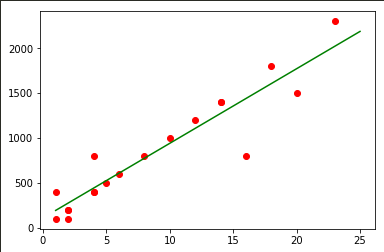
\includegraphics[scale=1]{LinearRegression.png}
\end{quote}
\textbf{Sử dụng Maximum Likelihood:}
\\
Ta nhận thấy giá gạo có thể tổng quát bởi công thức:
$$
    f(x) = a*x
$$
Áp dụng Maximum Likelihood với training data, chọn giá trị a = f(x)/x sao cho a có tần suất suất hiện nhiều nhất. Ta chọn được giá trị a = 100 và có thể kẻ đường thẳng f(x) = 100*x.
\begin{quote}
\centering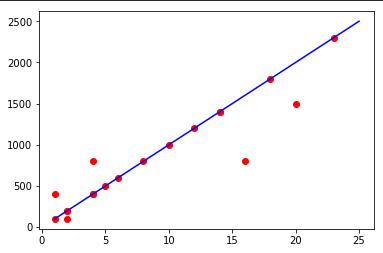
\includegraphics[scale=1]{MaximumLikelihood.png}
\end{quote}

\textbf{So sánh hai thuật toán}
\begin{enumerate}
    \item 
    \textbf{Linear Regression}
    \begin{enumerate}
        \item Khuyết điểm:
        \\ Ta có thể nhận thấy trong ví dụ trên, thuật toán Linear Regression cho kết quả khá "không chính xác" do dữ liệu có nhiễu nhiều.
        \\ Muốn cho thuật toán chính xác, ta cần có bước lọc nhiễu.
        \item Ưu điểm:
        \\ Mặc dù vậy, ở các bài toán mà không dễ dàng tìm được tham số có tần suất lớn nhất đủ lớn, thuật toán Linear Regression sẽ có ích hơn.
    \end{enumerate}
    \item
    \textbf{Maximum Likelihood}
    \begin{enumerate}
        \item Ưu điểm:
        \\Ở bài toán này, ta có thể thấy Maximum Likelihood thể hiện rất tốt và không bị ảnh hưởng bởi nhiễu.
        \\Ngoài ra, Maximum Likelihood rất dễ để hình dung và cài đặt.
        \item Nhược điểm:
        Maximum Likelihood là thuật toán chỉ nên áp dụng khi tần suất của một biến cố xảy ra đủ lớn, như ở ví dụ này tần suất của biến a khá lớn, nên có thể có độ chính xác cao. Ngoài ra Maximum Likelihood còn có thể mất độ chính xác khi các data tập trung thành 2 phần riêng biệt có số lượng bằng nhau hay số lượng data trong training data không đủ lớn dẫn đến hiện tượng overfitting.
    \end{enumerate}
    
\end{enumerate}
Ta có thể thấy Linear Regression và Maximum Likeklihood là 2 thuật toán cơ bản, dễ hiểu và dễ cài đặt, khá giống nhau khi được dùng để tìm ra mô hình chung của training data, nhưng mỗi thuật toán có ưu nhược điểm khác nhau phù hợp với từng trường hợp.

\textbf{Về Least-squares Method}
\\ Least-squares Method được sử dụng để tính hàm mất mát trong thuật toán Linear Regression vì tính đơn giản dễ hiểu và dễ giải đạo hàm của nó. Least-squares Method có mục tiêu là tìm bộ tham số để tổng các bình phương là nhỏ nhất.
\\ Còn trong Maximum Likelihood, ta có thể thấy ý nghĩa của thuật toán là tìm bộ tham số để số lượng các bình phương bằng 0 là nhiều nhất mà không cần quan tâm đến tổng của các bình phương ý.



\end{document}